%% =====================================================================
%%  DRAFT — ACM two-column (sigconf), anonymous review mode
%%  Kamer: archive-grounded generative-agent sandbox of Dutch parliament
%%  S1/S2/S3 numbers from runs/kamer/paper_exps.json (stable hash, PYTHONHASHSEED=0).
%% =====================================================================
\documentclass[sigconf,review,anonymous]{acmart}

\usepackage{booktabs}
\usepackage{multirow}
\usepackage{subcaption}
\usepackage{enumitem}
\usepackage{algorithm}
\usepackage{algpseudocode}
\usepackage{tikz}
\usetikzlibrary{positioning,arrows.meta,fit,backgrounds,shapes.geometric}

\newcommand{\tbd}[1]{\textcolor{red}{#1}}
\newcommand{\note}[1]{\textcolor{blue}{[\textbf{Note:} #1]}}
\newcommand{\sys}{\textsc{Kamer}}
\newcommand{\figph}[2]{%
  \fbox{\parbox[c][#2][c]{0.95\linewidth}{\centering\small\textcolor{red}{#1}}}}

\setcopyright{acmlicensed}
\copyrightyear{2027}
\acmYear{2027}
\acmDOI{XXXXXXX.XXXXXXX}
\acmConference[WWW '27]{The ACM Web Conference 2027}{2027}{City, Country}
\acmISBN{978-1-4503-XXXX-X/2027/06}

\begin{document}

\title[Countering Present-Day Bias in LLM Agents]{Countering Present-Day
Bias in LLM Agents: An Archive-Grounded Simulation of the Nineteenth-Century
Dutch Parliament}

\author{Anonymous Author(s)}
\affiliation{%
  \institution{Anonymous Institution}
  \city{City}
  \country{Country}}
\email{anonymous@example.com}

\renewcommand{\shortauthors}{Anonymous et al.}

%% =====================================================================
\begin{abstract}
LLM agents increasingly simulate societies, but they carry present-day
bias. Placed in a nineteenth-century parliament, they can use
twenty-first-century policy language and avoid the period's adversarial
register. Generative-agent sandboxes such as Smallville (Park et al., 2023)
do not correct this: any agent may speak anywhere, and believability is
judged by present-day readers. We present \sys{}, a sandbox of the Dutch
parliament that moves procedural constraints out of the language model and
into the world. Agents are seeded from attested speakers and their
recorded speech in the 1814--1899 proceedings. A \emph{role automaton} and
the standing orders decide who may act: only a recognised member may
speak, and journalists may watch from the press gallery but never take
the floor. An in-world stenographer writes a \emph{simulated Handelingen}
of recognised floor speech, which can be compared with the real, selective
record. With either the heuristic backend or \texttt{gpt-4o-mini}, the
simulated record, like the real one, contains no speech by journalists;
without the floor rules, journalists produce $4.3\%$ of it. Under the
transmission and allusion rules we encode, a resignation rumour reached
almost all members yet appeared in only $2\%$ of the record, so silence in
the Handelingen cannot by itself be read as ignorance. Present-day bias in
LLM-agent simulation therefore lies in the world as well as in the model's
language: an ungated sandbox writes a present-day assumption, that anyone
may speak anywhere, into every simulated record whatever the backbone.
Encoding the period's procedure removes this institutional bias and
confines the model's own bias to what agents say. When the model writes
every record line, a period prompt, the world, and archival retrieval with
filtering lower modern vocabulary from $10.5\%$ to $0.3\%$, but the
simulated debate remains far less adversarial than the archive.
\end{abstract}

% CCS concepts hidden for submission; restore for the camera-ready version.
% \begin{CCSXML}
% <ccs2012>
% <concept>
% <concept_id>10010147.10010341.10010349.10011810</concept_id>
% <concept_desc>Computing methodologies~Multi-agent systems</concept_desc>
% <concept_significance>500</concept_significance>
% </concept>
% <concept>
% <concept_id>10010405.10010469</concept_id>
% <concept_desc>Applied computing~Arts and humanities</concept_desc>
% <concept_significance>500</concept_significance>
% </concept>
% <concept>
% <concept_id>10003120.10003121</concept_id>
% <concept_desc>Human-centered computing~Human computer interaction (HCI)</concept_desc>
% <concept_significance>300</concept_significance>
% </concept>
% </ccs2012>
% \end{CCSXML}
% 
% \ccsdesc[500]{Computing methodologies~Multi-agent systems}
% \ccsdesc[500]{Applied computing~Arts and humanities}
% \ccsdesc[300]{Human-centered computing~Human computer interaction (HCI)}

\keywords{generative agents, sandbox simulation, large language models,
digital history, parliamentary proceedings, computational social science}

\begin{teaserfigure}
  \centering
  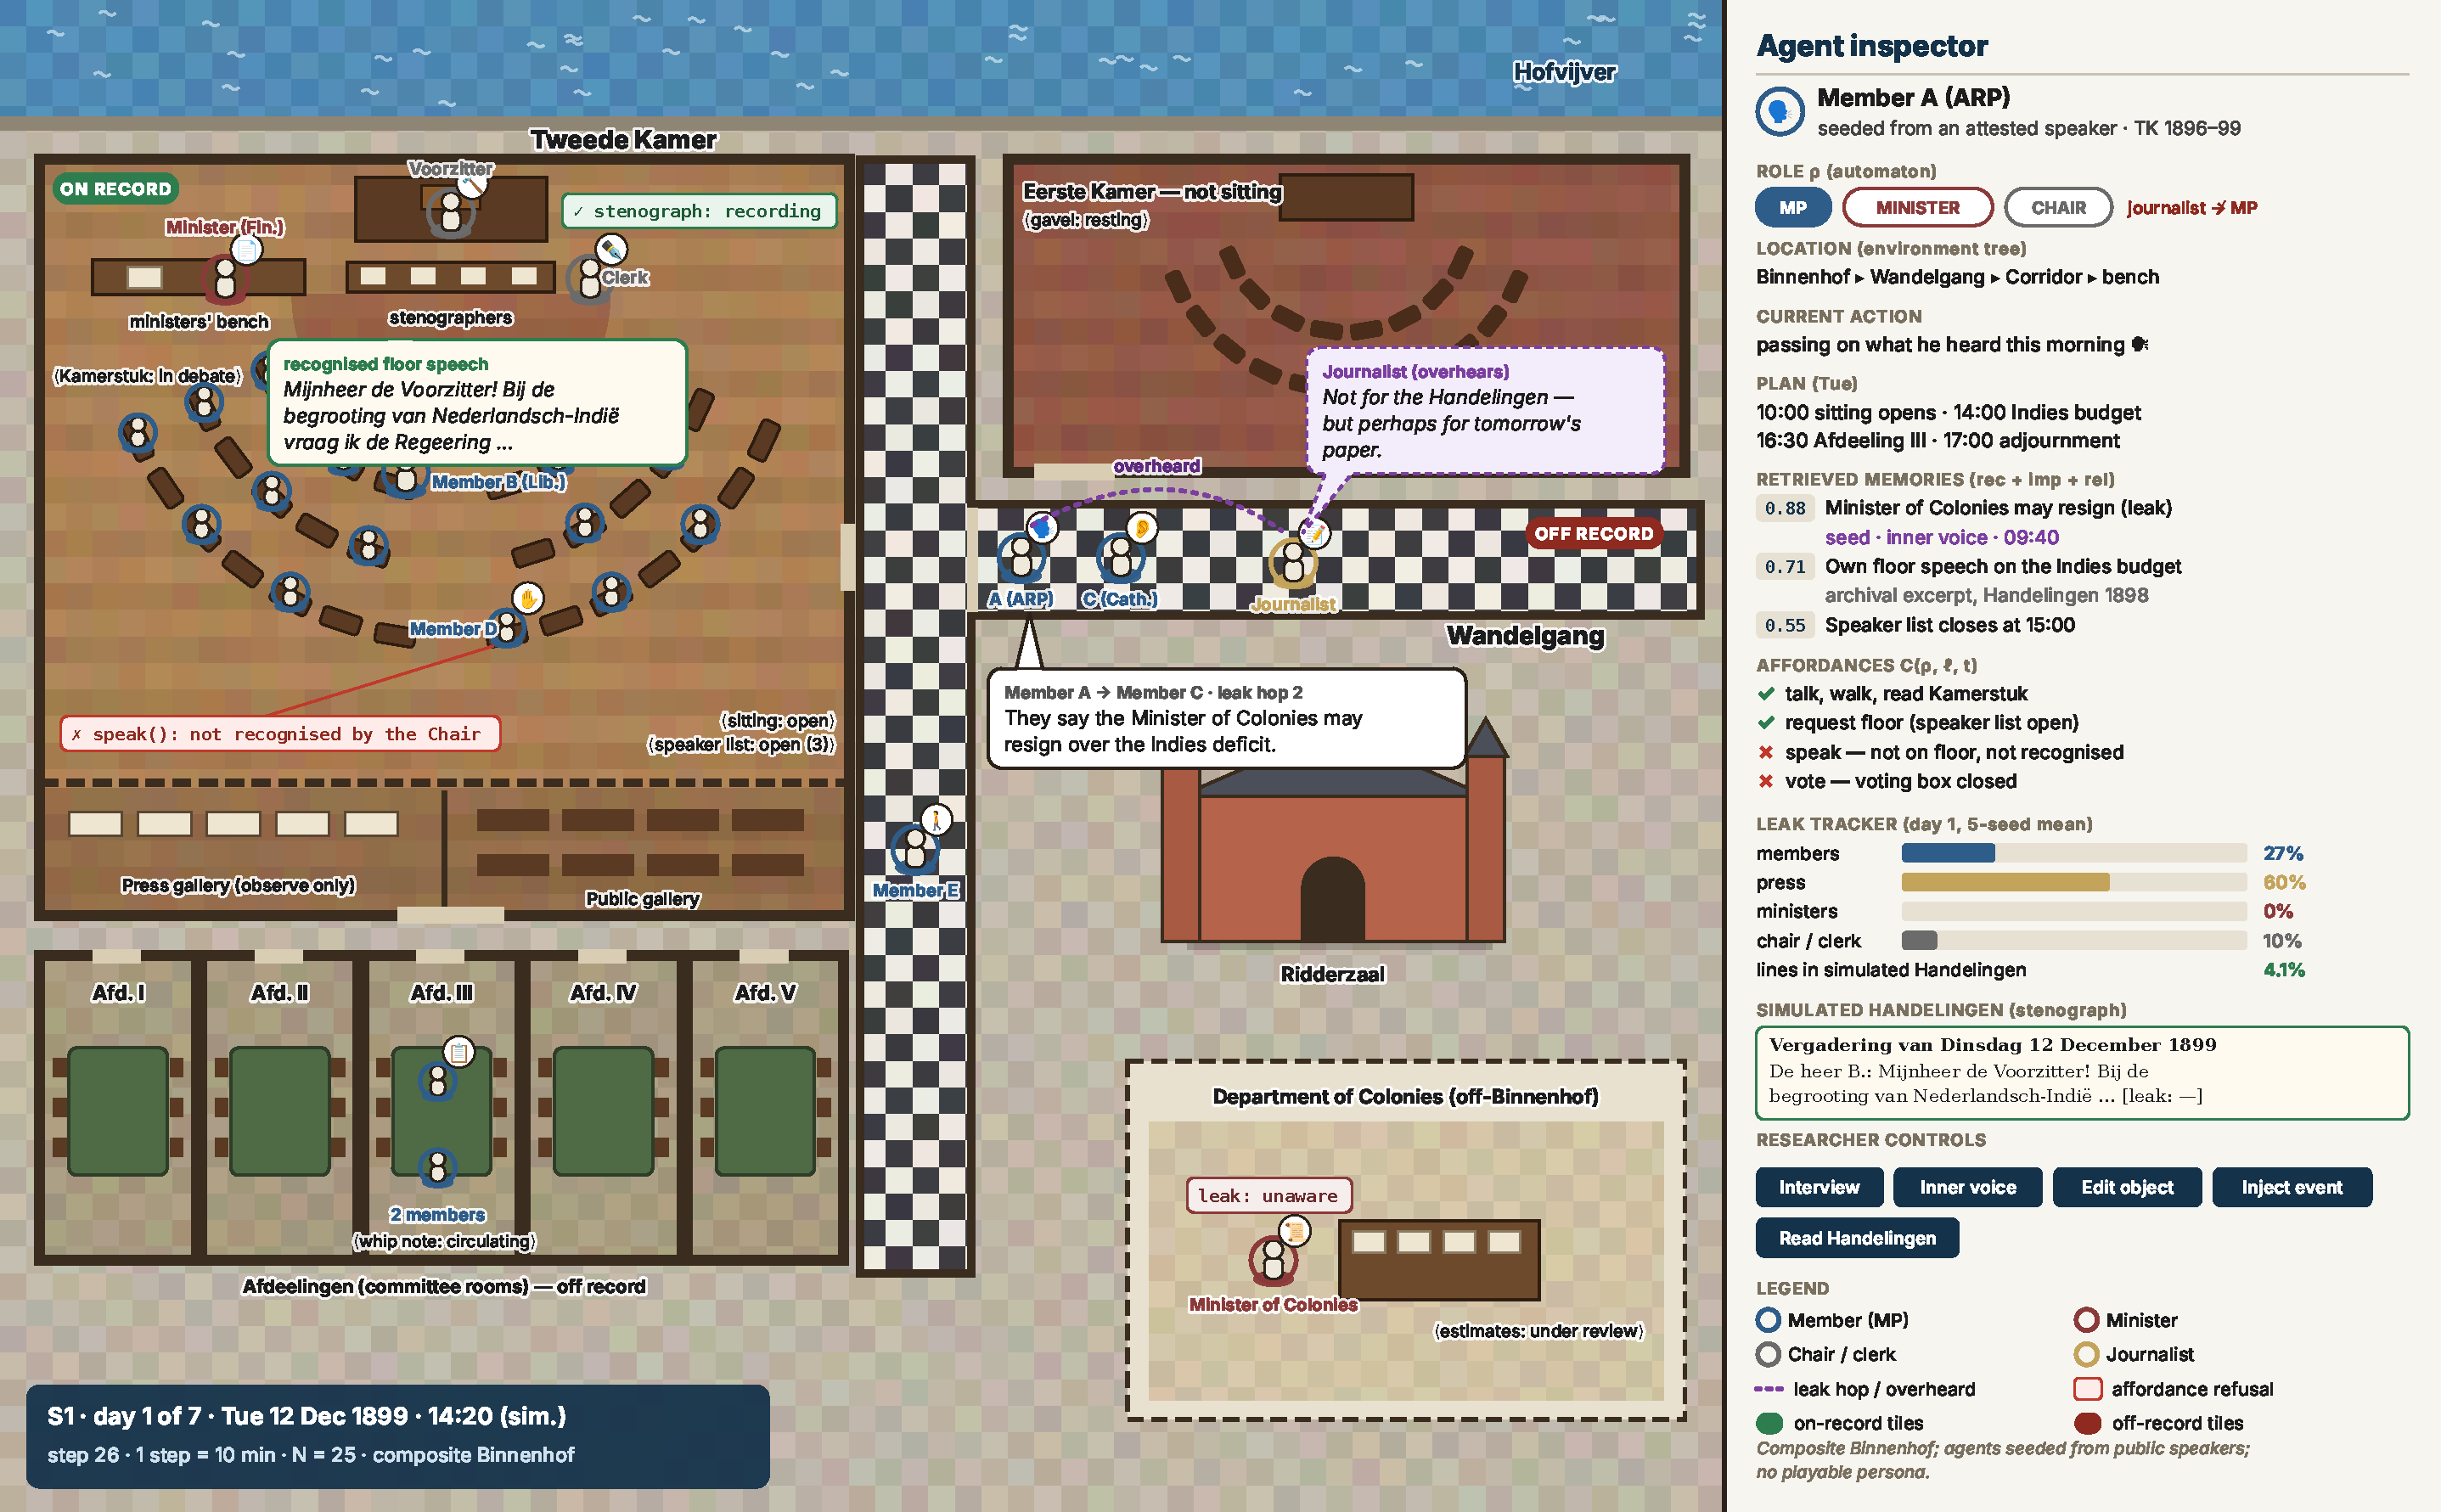
\includegraphics[width=\textwidth]{figure/kamer_sandbox.pdf}
  \caption{The \sys{} sandbox on day~1 of a simulated week in December 1899
  ($N{=}25$). A recognised member speaks on the East Indies budget while an
  unrecognised member is refused the floor; in the wandelgang, a rumour that
  the Minister of Colonies may resign passes between members and reaches a
  journalist but not the Handelingen. Right: the agent inspector (role,
  location, affordances, memories, leak tracker, researcher controls).}
  \Description{A top-down map of a composite Binnenhof with the Tweede Kamer
  floor, wandelgang, committee rooms, press gallery and an agent inspector.}
  \label{fig:teaser}
\end{teaserfigure}

\maketitle

%% =====================================================================
\section{Introduction}
\label{sec:intro}

Historians study processes they cannot observe directly. How did news
spread through a city? Why did one group gain influence while another lost
it? What did people know but never write down? The sources that survive
record outcomes, not the processes behind them, and they record only part
of what happened~\cite{trouillot1995silencing}. Questions about
alternatives are harder still: no archive shows what would have happened
if a rule had been different~\cite{ferguson1997virtual}.
Simulation can help. A historian can model the people of a period and the
rules they followed, run the model, and check whether a proposed
explanation produces the patterns found in the
archive~\cite{epstein1996growing,epstein2006generative,gavin2014abm}.
Agent-based models have been used in this way to study settlement,
exchange, and population history~\cite{axtell2002population,romanowska2021abm}. Their agents, however, follow
hand-written rules and cannot talk, so they cannot represent the debates,
letters, and rumours through which much of history happened.

Generative agents~\cite{park2023generative} remove this limitation. In
Smallville, 25 agents driven by large language models (LLMs) perceive
their surroundings, store observations in a memory stream, reflect, and
plan. Together they produce emergent social behaviour such as information
diffusion and the coordination of a Valentine's Day party, in an
interactive sandbox where a user can watch, interview, and intervene.
Later work has scaled such societies to more than a thousand
agents~\cite{al2024projectsid,piao2025agentsociety}. Using such agents to
simulate the past, however, runs into a problem that matters for any use
of LLM agents: present-day bias. A language model learns mostly from
contemporary Web text, so its agents tend to speak, judge, and act as
people do today~\cite{santurkar2023opinions,wang2025identity}. In a
simulation of the present this bias is hard to see; in a simulation of the
past it becomes visible as anachronism and can be checked against the
historical record. Historical simulation is therefore a demanding test bed
for measuring and countering present-day bias in LLM agents.

Parliaments are a good case because their debates are unusually well
recorded. For the Netherlands, the \emph{Handelingen der Staten-Generaal}
cover every sitting of the States General since 1814 and are published on
the Web as PoliticalMashup XML under
CC0~\cite{marx2012dutchparl,marx2010dutchparl}. They are, however, an
\emph{official} record: produced under standing orders, edited, and silent
about the corridor. Simulating such a parliament with generative agents
raises three challenges. First, present-day bias, which historians call
presentism, appears in concrete ways: simulated members speak
twenty-first-century policy language, refuse the adversarial register of
nineteenth-century debate~\cite{wang2025identity,bender2021parrots}, or
call themselves English-style ``MPs'' rather than members of a particular
chamber, and a persona prompt alone cannot rule this out.
Second, existing sandbox worlds are \emph{ungated}: any agent may speak
anywhere, so nothing stops a journalist from taking the floor, and
procedure is left to the model's willingness to role-play. Third, existing
sandboxes are validated against \emph{present-day} judgements of
believability, whereas a historical simulation must be checked against an
archive that is itself selective: the Handelingen record the floor, not
the wandelgang (the lobby corridor).

We address these challenges by moving historical constraints out of the
language model and into the world, where they can be inspected and
tested. We implement this design in \sys{}, an archive-grounded generative
agent sandbox of the nineteenth-century Dutch parliament, set in a
composite Binnenhof, the parliamentary complex in The Hague
(Figure~\ref{fig:teaser}). The archive supplies who may appear and how
they spoke: agents are seeded from attested speakers and their recorded
speech in the 1814--1899 proceedings. Institutions decide who may act: as
in Smallville, the world is a 2D map backed by an environment tree, but
every action in that tree is gated by the agent's role (Chair, member,
minister, clerk, journalist), the Reglement van Orde (the standing
orders), and whether the sitting is open, so a journalist cannot take the
floor however the model is prompted. The archive's own selection becomes
the validation target: corridor talk travels with provenance and
distortion, but an in-world stenographer writes only recognised floor
speech, producing a simulated record that can be compared with the real
one. Researchers can pause the sandbox, step through a sitting, inspect
agents, and interview them. Other interventions are logged, but only
opening a sitting currently changes what agents do
(Appendix~\ref{app:interface}).

Experiments with \sys{} support this design. A historian judged \sys{}'s
interview answers more plausible for a late-1890s member than those of a Smallville-style baseline (17 wins,
8 losses, 11 ties). Institutional outcomes, in turn, did not depend on the
backbone. Like the real Handelingen, the simulated record contains no
speech by journalists; without the floor rules, journalists produce
$4.3\%$ of it, and replacing the heuristic backend with
\texttt{gpt-4o-mini} changes neither figure. The record also diverged
sharply from what parliament knew: under the transmission and allusion
rules we encode, a resignation rumour reached almost all members within a
week but appeared in only $2\%$ of the simulated record
(\S\ref{sec:results}). When the model writes every record line, a period
prompt, the world, and archival retrieval with filtering lower modern
vocabulary from $10.5\%$ to $0.3\%$, but the simulated debate remains far
less adversarial than the archive. These results suggest that institutional outcomes
are better secured by encoding procedure in the world than by relying on
the language model, and that
silence in the Handelingen cannot by itself be read as ignorance.

In summary, we make the following contributions:
\begin{itemize}[leftmargin=*,nosep]
  \item \textbf{Countering present-day bias outside the language model.} A
  design that places historical constraints in the archive and in the world
  rather than in the prompt alone, implemented in \sys{}: a tile world of
  the Binnenhof whose environment tree, object states, and affordances
  encode the standing orders of both chambers, together with a
  parliamentary role automaton. This procedural gating holds regardless of
  the backbone (\S\ref{sec:world}, \S\ref{sec:agents}).
  \item \textbf{An archive-to-sandbox pipeline and a simulated
  Handelingen.} We build the world, its rules, and a population of attested
  public speakers, seeded with their recorded speech, from PoliticalMashup
  XML (8{,}745 sittings and 138{,}214 speeches in the 1814--1899 slice). An
  in-world stenographer records only recognised floor speech, so that the
  simulation can be compared with \emph{what the archive could have
  recorded} (\S\ref{sec:pipeline}, \S\ref{sec:calibration}).
  \item \textbf{Evaluation.} Three experiments: a simulated one-week
  sitting in December 1899 (S1), with corridor-versus-floor leak diffusion,
  ablations of the standing orders and the rumour network, and a backbone
  check with \texttt{gpt-4o-mini}; a selection-aware comparison with
  held-out Handelingen from 1890--1899 (S2); and an intervention on Chair
  strictness (S3). A presentism audit, in which the model writes every
  record line, separates the effects of prompt, world, and guards, and a
  historian ranks agent interviews
  (\S\ref{sec:experiments}--\S\ref{sec:results}).
\end{itemize}

%% =====================================================================
\section{Related Work}
\label{sec:related}

\paragraph{Generative agents and social simulation.} Classical
agent-based models (ABMs) explain macro phenomena from local
rules~\cite{schelling1971dynamic,epstein1996growing}; the generative
standard requires that a candidate explanation actually grow the
phenomenon~\cite{epstein2006generative}. Social
simulacra~\cite{park2022social} first used LLMs to populate prototypes of
online communities, and Generative Agents~\cite{park2023generative} gave
25 agents in Smallville a memory stream, reflection, and planning. Later
systems add needs, emotions, and desires~\cite{wang2023humanoid,wang2025desire},
ground behaviour in physical environments~\cite{wu2025indoorworld,liang2025virtual},
and scale to cities~\cite{bougie2025citysim} and
societies~\cite{al2024projectsid,piao2025agentsociety}. LLMs also simulate
survey respondents~\cite{argyle2023outofone,aher2023turing}, economic
actors~\cite{horton2023homosilicus}, and social-network
users~\cite{gao2023s3,tornberg2023simulating} (see~\cite{gao2024llmabm}
for a survey). Closer to our setting, LLM agents have simulated states on
the road to the world wars~\cite{hua2023waragent} and deliberation in a US Senate
committee~\cite{baker2024senate}. In Concordia~\cite{vezhnevets2023concordia},
a game-master agent turns the actions that agents describe into outcomes
in the world. Work on electronic institutions~\cite{esteva2001electronic}
and the grammar of institutions~\cite{crawford1995grammar} specifies the
roles, rules, and protocols of interaction outside the agents themselves.
\sys{} adopts the sandbox design of Generative Agents (tile map,
environment tree, memory stream) but, like these institutional approaches,
enforces its standing orders in the world rather than through a model. It also follows the
generative standard: its claims concern which institutional rules suffice
to produce the patterns in the record (\S\ref{sec:discussion}).

\paragraph{Present-day bias and behavioural fidelity.} LLMs trained on
contemporary Web text reproduce the views of particular present-day
populations: some US demographic groups~\cite{santurkar2023opinions}, the
USA and parts of Europe~\cite{durmus2023global}, English-speaking and
Protestant European countries~\cite{tao2024cultural}, and WEIRD
populations more generally~\cite{atari2023which}. Simulated personas can
flatten identity groups~\cite{wang2025identity}, exaggerate them into
caricature~\cite{cheng2023compost}, and encode representational
harms~\cite{bender2021parrots}, and convincing simulated behaviour may
still be unfounded~\cite{ziems2024css}. Studies of behavioural fidelity
compare simulations with real data: LLMs miss human response biases in
surveys~\cite{tjuatja2024biases,bisbee2024synthetic}, are more cooperative
than people in dialogue~\cite{ivey2024real,zhou2026sim2real}, and struggle
to reproduce real behaviour over long
horizons~\cite{li2025digitaltwins,chen2026traces,cheng2026longhorizon},
while agents built from qualitative interviews replicate their
participants' survey answers~\cite{park2024thousand}. Role-playing agents
can be trained to imitate historical figures~\cite{shao2023characterllm},
and historical LLMs trained on period corpora have been proposed as
simulated participants from past societies~\cite{varnum2024historical}. In a
nineteenth-century parliament, whose culture prized oratory and principled
debate~\cite{tevelde2015sprekende}, present-day bias appears as
anachronistic vocabulary, sanitised conflict, and members who
``cooperate'' instead of opposing. \sys{} measures fidelity against a
selective past record and, rather than retraining the model, moves
procedure out of it and audits the text it still writes
(\S\ref{sec:results}).

\paragraph{Parliamentary records as selective archives.} DutchParl and
PoliticalMashup encode the Handelingen as proceedings XML with speaker,
role, party, and house metadata~\cite{marx2010dutchparl,marx2012dutchparl}.
The scans come from Staten-Generaal Digitaal (Koninklijke Bibliotheek).
Comparable corpora cover other
parliaments~\cite{erjavec2023parlamint,rauh2020parlspeech}.
NLP on historical proceedings must cope with OCR noise and spelling variation~\cite{ehrmann2023ner}. Such
records are not transparent windows onto
events~\cite{trouillot1995silencing,stoler2009archival}. Studies of the
British Hansard show that the official report drops features of spoken
interaction, changes wording, and understates the force of
exchanges~\cite{slembrouck1992hansard,mollin2007hansard}.
The Handelingen likewise omit what the Chair did not recognise and what
members chose not to say on the floor, and the Tweede Kamer of the
period built its authority through such rules and
practices~\cite{turpijn2008mannen}. \sys{} uses the corpus both as a
\emph{seed} (personas, speech style, sitting calendars) and as a
\emph{validation target} (who spoke, for how long, on which topics, and in
which house), and treats its selection as a design constraint: the sandbox
generates hypotheses about \emph{processes}, including the process that
produced the record, and never offers testimony about unrecorded inner
lives.

%% =====================================================================
\section{The \sys{} Sandbox}
\label{sec:sandbox}

The sandbox has three parts, which answer the three challenges of
\S\ref{sec:intro}. An archive-to-sandbox pipeline (\S\ref{sec:pipeline})
supplies the world's rules and a population of attested speakers. The
world (\S\ref{sec:world}) and the role-constrained agents
(\S\ref{sec:agents}) decide who may act, and an in-world stenographer
turns recognised floor speech into a simulated record that is compared
with the real one (\S\ref{sec:calibration}). Algorithm~\ref{alg:step}
(Appendix~\ref{app:alg}) summarises one step.

\subsection{Archive-to-sandbox pipeline}
\label{sec:pipeline}

\paragraph{Sources.} We use the non-semanticized PoliticalMashup release of
the Dutch parliamentary proceedings~\cite{marx2012dutchparl}: one XML
document per sitting from 1814 to April 2012, released under CC0. Our
working slice covers \textbf{1814--1899}: 8{,}745 sittings, of which
6{,}340 are Tweede Kamer sittings (\texttt{pm:house="commons"}), 2{,}036
are Eerste Kamer sittings (\texttt{senate}), and 369 are early or
unlabelled meetings. Of these, 7{,}348 files contain at least one
\texttt{speech} element, yielding \textbf{138{,}214} speaker-attributed
speeches (Table~\ref{tab:corpus}, Appendix~\ref{app:tables}).
PoliticalMashup records 852 distinct \texttt{pm:member-ref}
identifiers; raw \texttt{pm:speaker} strings are far more numerous because
of OCR variation. Role attributes on speech elements are dominated by
\texttt{mp}, followed by \texttt{government} and \texttt{chair}. Party
references in the later nineteenth century include liberals,
conservatives, anti-revolutionaries, Catholics, and, by the 1890s, the
SDAP. The post-1899 portion of the corpus is left to future work.


\paragraph{Event extraction.} A schema-constrained parser reads each
sitting's Dublin Core header (date, title, house, legislative period) and
every \texttt{speech} element (speaker, role, function, party, member-ref,
text). OCR noise is retained as a property of the archive: unless a
member-ref is present, personas inherit the \emph{documented} name string
rather than a cleaned modern spelling. Every field keeps its source
attribution.

\paragraph{From records to world.} Historians translate the Reglement van
Orde and secondary literature on the Staten-Generaal into
(i)~affordance rules (who may speak, recognise, vote, or sit in the
gallery), (ii)~object schedules (sitting hours, speaker lists, budget
debates), and (iii)~the layout of the environment tree $\mathcal{T}$
(\S\ref{sec:world}; 6 areas, 15 subareas, and 7 objects in the simulated
Binnenhof).

\subsection{World: tile map and environment tree}
\label{sec:world}

The world is a 2D tile map of a composite Binnenhof
(Figure~\ref{fig:teaser}). Its layout and institutions are calibrated to
the late-nineteenth-century Staten-Generaal, but it reproduces no single
historical floor plan. Following Smallville~\cite{park2023generative}, the
map is backed by an \emph{environment tree}
\[
\mathcal{T}:\ \textsf{Binnenhof}\ \triangleright\ \textsf{Area}\ \triangleright\
\textsf{Subarea}\ \triangleright\ \textsf{Object},
\]
e.g.,\\ \textsf{Binnenhof\,$\triangleright$\,Tweede Kamer\,$\triangleright$\,Right benches\,$\triangleright$\,kamerstuk}
or
\textsf{Binnenhof\,$\triangleright$\,Wandelgang\,$\triangleright$\,Corridor}.
The root node, Binnenhof, represents the whole world; its children are
areas, their children are subareas, and the leaves are objects. The areas
are the Tweede Kamer (chair's dais, stenographers' table,
griffier's (clerk's) desk, ministers' bench, left and right benches, aisle,
tribune), the Eerste Kamer (its own chair, floor, and benches), the
wandelgang, committee rooms (afdeelingen), the press gallery, and ministers'
rooms. Each tile carries an \emph{on-record} or \emph{off-record} tag,
which determines whether the stenographer may write, and a house tag
(\texttt{commons} or \texttt{senate}).

\paragraph{Two chambers.} The Staten-Generaal has been bicameral since 1815.
The directly elected Tweede Kamer amends and initiates bills and decides
whether cabinets stand. The Eerste Kamer, elected by the Provinciale
Staten, sits far less often and may only accept or reject
bills~\cite{pdc2024kamers}, yet between 1888 and 1918 it several times
blocked cabinets that held a Tweede Kamer majority. \sys{} therefore treats house membership as
an institutional attribute rather than a label. A Kamerlid of the Tweede
Kamer has no floor rights in the Eerste Kamer; ministers, who appear in
both houses, do; and \texttt{move\_amendment} is undefined on senate tiles.
Although the simulated week has only Tweede Kamer sittings, the Eerste Kamer is present on the map
and in the affordance layer, so that ``lid der Staten-Generaal'' (member of
the States General) is never an admissible self-description.

\paragraph{Stateful objects.} Every leaf of $\mathcal{T}$ is an object with
a natural-language state that agents perceive and actions change
(Table~\ref{tab:objects}, Appendix~\ref{app:tables}). Objects make
procedure concrete: the speaker list
is open or closed, the gavel opens and adjourns the sitting, the stenograph
is idle or recording, and a Kamerstuk (parliamentary paper) moves from
tabled to in debate to voted.

\paragraph{Time, engine, and interface.} One simulation step corresponds
to $10$ minutes of in-world time.
Sittings open on weekdays at 10:00 and adjourn at 17:00, matching the
rhythm of the Handelingen. \sys{} follows the server--client design of
open-source Smallville implementations~\cite{smallvillerepo}: a simulation
server holds the environment tree, object states, and agent memories,
advances the world with an \texttt{updateState} call, and exposes this
state over a REST API. Researchers can
pause the world, step through it, inspect agents, and interview them.
Adding a memory, editing an object state, and injecting an event are also
logged, but of these only opening a sitting changes what agents do. No
agent can be controlled in the first person (Appendix~\ref{app:interface}).

\subsection{Role-constrained agents}
\label{sec:agents}

Each agent is seeded from the archive and asked to speak in period Dutch
(\S\ref{sec:personas}). At every step it records what it perceives and
attempts an action chosen by its role and the sitting schedule
(\S\ref{sec:memory}); the role automaton and the affordance layer then
decide whether the action succeeds (\S\ref{sec:gating}); and floor
speech, conversation, and rumours carry information between agents
(\S\ref{sec:communication}). Appendix~\ref{app:day} traces one simulated
day through these rules (Figure~\ref{fig:day}).

\subsubsection{Personas and period language}
\label{sec:personas}
For the simulated week, we sample $N{=}25$ agents from attested speakers
in Tweede Kamer sittings of 1896--1899, filtered to the offices held in
December 1899: Gleichman as Chair, Cremer and Goeman Borgesius as
ministers of the Pierson cabinet, Arntzenius as griffier, one journalist,
and 20 members. Each agent is seeded with a short persona and up to three
excerpts of the person's actual public speech. Unlike the Smallville
seed descriptions, which cover occupation, family, and relationships, the
seed holds only public office, house, party, and attested speech; no
private life is instantiated (Appendix~\ref{app:examples} shows Kuyper's
seed). The persona is prepended to every LLM
prompt, and the opening of the first excerpt is reused verbatim when the
agent speaks on the floor without an LLM completion. Agents identify as
Kamerlid, minister, or Voorzitter (Chair) \emph{der Tweede Kamer} (or
Eerste Kamer), never as an English ``MP'' of an undifferentiated
Staten-Generaal. The journalist is the only role not drawn from a
\texttt{speech} element: the Handelingen do not record the press gallery,
and the sandbox includes the role for that reason. The griffier is a
named office-holder (Arntzenius, in office 1888--1920); the stenographer is
a separate role that writes the simulated record (\S\ref{sec:calibration}).

The system prompt of the LLM backbone asks
for late-nineteenth-century Dutch and lists period forms such as
\emph{thans}, \emph{eene}, \emph{hetgeen}, and \emph{Nederlandsch}; the
Smallville-style baseline asks only for ``period Dutch''. The presentism
audit (\S\ref{sec:experiments}) adds two guards: archival retrieval puts
the two most similar opening passages of 1860--1889 Tweede Kamer speeches
(the calibration slice, never the holdout) in each prompt as a register
and spelling reference, and an anachronism filter regenerates a draft once
if it contains a term from one half of the modern lexicon, keeping the
other half for auditing. Neither guard is active in S1--S3.

\subsubsection{Memory and action selection}
\label{sec:memory}
Each agent keeps a memory stream
of observations, conversation, refusals, and its own speeches, each entry
with a fixed importance by type. At every step the agent records what it
perceives: its location, whether the sitting is open, who holds the floor,
the objects around it, and who else is present. Such observations make up
about 99\% of the roughly 4{,}000 entries an agent accumulates in a week.
When the language model writes an utterance, its prompt contains the
agent's persona and six most recent memories, which typically cover only
the last 10 to 20 simulated minutes; interviews use the eight most recent.
A rumour heard earlier in the day has therefore usually left this window:
in the day of Figure~\ref{fig:day}, the rumour Seret heard at 09:10 lies
49 entries back when he speaks at 11:30. Whether a prompt mentions the
rumour is decided by the rumour channel instead. An agent that has
received the rumour gets a fixed sentence stating it and may allude to it
on the floor; an agent that has not is told not to invent one. Unlike
Generative
Agents~\cite{park2023generative}, \sys{} does not rank memories by
recency, importance, and relevance, does not synthesise reflections, and
does not ask the model to plan. Where an agent goes and which action it
attempts are set by rules tied to its role and to the sitting schedule.
During a sitting,
members and ministers sit on their benches and ask for the floor; the
Chair opens and adjourns the sitting and, whenever nobody holds the floor,
gives it to the next member or minister in rotation; and the journalist
sits at the press-gallery desk. Outside sittings, members gather in the
wandelgang or a committee room, and ministers withdraw to their ministry
in the evening. The language model therefore decides what an agent says,
never where it goes or whether it may speak.

\subsubsection{Roles and affordances}
\label{sec:gating}
Each agent holds one role at a time: Chair,
Kamerlid, minister, griffier, journalist, or visitor in the public gallery.
Each role belongs to the Tweede Kamer (\texttt{commons}), the Eerste Kamer
(\texttt{senate}), or both. We write $\rho_i^t$ for the role of agent $i$
at step $t$. The role automaton $\mathcal{A}$ lists the changes of role
that the historical institution allows, together with the conditions under
which each may occur: a member may become a minister (by appointment) or
Chair (by election), and a minister may return to the benches, but a
journalist cannot become a member by walking onto the floor. An agent can
change role only through one of these transitions, and only when its
condition holds in the current state of the sandbox. No appointment or
election is scheduled in the simulated week, so no transition occurs in the reported runs.
Procedure on the floor is enforced by the affordance layer, not by the
LLM's willingness to role-play a Voorzitter.

Every attempted action is checked against the
affordance set $\mathcal{C}(\rho_i^t,v,t)$ of the agent's current node $v$,
which encodes the Reglement van Orde as a function of the agent's role and
house, the node's tags, and the state of the sitting. An agent may
\emph{want} to speak, but it can \emph{act} only when the Chair has
recognised it, the sitting is open, and its role permits the act; in an
afdeeling, members speak without recognition and off the record. A
rejected action produces a structured refusal, such as ``Mijnheer de
Voorzitter heeft u het woord nog niet gegeven'' (roughly, ``the Chair has
not yet given you the floor'') or, for the journalist, ``De perstribune
heeft geen spreekrecht op de vloer'' (``the press gallery has no right to
speak on the floor''). The refusal is written to the agent's memory, and
the agent waits for the rest of the step (Algorithm~\ref{alg:step},
Appendix~\ref{app:alg}).

\subsubsection{Communication}
\label{sec:communication}
Agents communicate through three channels,
which differ in who can hear and what is recorded. \emph{Floor speech}
requires recognition. When the Chair gives the floor (``Het woord is aan
den heer Kuyper''), the recognised member addresses the Chair, and the
stenographer writes the utterance into the simulated Handelingen. Other
agents perceive who holds the floor but not the content of the speech.
Under the heuristic backend, a floor speech is the opening of the
speaker's first attested excerpt. A member who knows of the rumour ends
its floor speeches with a fixed allusion (``Zonder de geruchten uit de
wandelgang te willen bevestigen, vraag ik of de begrooting sluit'') on
about one sitting day in $\max(3,12s)$, where $s$ is the Chair strictness
($s=1$ by default).
\emph{Conversation} happens wherever agents share a subarea. At 09:00,
11:00, 13:00, 17:00, and 18:00, each agent picks one co-present agent at
random and, with probability $0.40$ in the wandelgang, $0.12$ in other
off-record places, and $0.04$ on the floor, addresses one remark to it.
The remark is generated by the language model from the speaker's persona
and six most recent memories (or is a fixed sentence under the heuristic
backend) and is stored in the memories of both agents; there is no
multi-turn exchange. Agents in the wandelgang also show short asides in
their bubbles, which are displayed but not remembered. \emph{Rumours}
travel on a separate, structured channel. A rumour is a set of facts (who,
what, how much, where, and when) with a provenance chain of hops. At each
encounter, the speaker may pass on a rumour it knows, with probability
$0.28$ in the wandelgang, $0.10$ in other off-record places, and $0.02$ on
the floor; in the wandelgang it is multiplied by $0.35$ for hearers who
are ministers, the Chair, or the griffier, and is at least $0.55$ for the
journalist as hearer. With probability $d$, the corridor distortion ($0.18$ by
default), one fact changes at the hop, for example ``this week'' becoming
``after the vote''. The hearer perceives the rumour as ``[speaker] told
me: \ldots'' and may learn the places it names.
Appendix~\ref{app:examples} gives an example remark from a
\texttt{gpt-4o-mini} run.

\subsection{Simulated Handelingen}
\label{sec:calibration}

While the sitting is open, the
stenographer writes each speech by the recognised member or minister on
the floor into the simulated Handelingen $Y^t$. Corridor talk, committee
speech, and the journalist's notes never enter it. In the reported runs,
the Chair's recognitions and rulings are logged as events but not written
as lines, so the simulated record contains no speech by the Chair. This
in-world process mirrors the archive's selection, formalised below.

\paragraph{Selection-aware comparison.} Let $x$ denote the features of an
event such as a speech, a leak, or a
vote (speaker role, party, house, topic, duration), and let
$P^\theta_{\text{sim}}$ be the distribution of simulated events under
parameters $\theta$ (Chair strictness, corridor distortion, willingness to
allude to a matter on the floor, \ldots). The real Handelingen record an
event only if it was spoken on the floor after recognition. This happens
with a propensity $\pi(x)$ that depends, for example, on whether the Chair
called the member and whether the member chose to put the matter on the
record, so that
\begin{equation}
P_{\text{arch}}(x)=\frac{\pi(x)\,P_{\text{true}}(x)}{\int \pi(x')\,P_{\text{true}}(x')\,dx'}.
\label{eq:selection}
\end{equation}

Equation~\eqref{eq:selection} has a direct consequence for comparing a
simulation with the archive.
Whenever some events are more likely to be recorded than others, the
archive over-represents the former, so a simulation tuned until everything
its agents do matches the archive is tuned to the wrong target: it
reproduces the record, not the events behind it. Corridor talk is the
clearest case, since it is common in the world but absent from the record.
The remedy is to compare like with like. Instead of matching all simulated
events, we match only the events that the simulated stenographer records,
whose distribution we denote $\tilde P^\theta_{\text{sim}}$; these pass
through the same filter $\pi$ as the real archive. If $\pi$ is specified
correctly and the simulator can represent the historical process, matching
$\tilde P^\theta_{\text{sim}}$ to $P_{\text{arch}}$ recovers the
distribution of events that actually took place.

In \sys{}, $\pi$ is set by the stenographer's rule (record iff the
location is on-record, the sitting is open, and the speaker is recognised
or is the Chair) together with the rule by which members allude to rumours
on the floor (\S\ref{sec:communication}). The same comparison can serve
as a calibration objective for $\theta$ (Appendix~\ref{app:calib}); in
this paper we do not fit $\theta$ but evaluate the default parameters
against held-out Handelingen (\S\ref{sec:experiments}).

%% =====================================================================
\section{Experimental Setup}
\label{sec:experiments}

\paragraph{S1 (one-week sitting).} S1 runs $N{=}25$ agents, the scale of
Smallville, through a composite Tweede Kamer week in December 1899. Eerste
Kamer tiles exist and are gated, but no senate sitting opens during this
week. We seed a corridor leak and compare \sys{} with four ablations:
\textbf{GA}, which disables the affordance layer, the automaton, and the
rumour channel and uses a free-sandbox prompt (``Anyone may speak to
anyone''), as in an ungated Smallville-style
world~\cite{park2023generative}; \textbf{--affordance};
\textbf{--automaton}; and \textbf{--rumour}.

\paragraph{S2 (selection-aware fidelity).} We hold out Tweede Kamer
speeches from 1890--1899 (731 sittings and 20{,}166 speeches; role mix
$64\%$ MP, $18\%$ government, $18\%$ chair, $0\%$ journalist) and use
1860--1889 (72{,}112 speeches) as the calibration slice. No parameter of
\sys{} is fitted to this slice; it serves the Rule-ABM baseline. We compare
the role mix (Jensen--Shannon divergence) and the share of official lines
spoken by a journalist. Besides GA, we include two baselines:
\textbf{Rule-ABM} replays the empirical 1860--1889 role
mix~\cite{epstein1996growing}, and \textbf{naive calibration} counts
corridor dialogue as if it were Handelingen (\S\ref{sec:calibration}).

\paragraph{S3 (intervention).} S3 scales Chair strictness by
$\{0.25,0.5,1,2,4\}$ relative to the default, crosses it with corridor
distortion $\{0.05,0.18\}$, and reports the floor-mention rate of the leak.
Strictness $s$ enters the model in two places: it sets the heuristic
allusion rate (\S\ref{sec:communication}), and for $s\geq2$ the Chair gives the
floor only on every $s$-th step.

\paragraph{Backends and seeds.} S1 (including its ablations), S2, and S3
use the heuristic backend, in which floor speeches are attested excerpts and conversation remarks are
fixed sentences (seeds $\{7,11,19,29,31\}$). All reported runs set
\texttt{PYTHONHASHSEED=0}, and bench seating and the heuristic allusion
rule use a process-independent hash. A backbone check reruns the
S1 \texttt{full} and \texttt{ga} conditions with \texttt{gpt-4o-mini}
(seeds $\{7,11,19\}$). Each run had a budget of 400 completions, mostly
spent on corridor asides, after which agents fell back to heuristic
utterances; at most 20 of the 205 record lines per seed are model text.

\paragraph{Presentism audit.} A separate \texttt{gpt-4o-mini} run (seeds
$\{7,11,19\}$) uses the model for every floor, corridor, and interview
turn, so every record line is model text, and agents hear the previous
floor speech. Four conditions separate world, prompt, and guards:
\textbf{GA}; \textbf{GA + period prompt} (Smallville-style world, \sys{}
system prompt); \textbf{\sys{} world} (no guards); and
\textbf{\sys{} + guards}. We score distinct completions against the
1890--1899 holdout (14{,}731 speeches, first 480 characters): the share
with a term from a 38-term Dutch and English modern lexicon (16 terms
attested in the holdout removed), with an adversarial marker (a challenge
cue, or a reference to another speaker with a contrastive conjunction),
and with a consensus cue. Intervals are 95\% cluster-bootstrap intervals
over seeds and turns.

\subsection{End-to-end evaluation}
\label{sec:eval-e2e}
\textbf{Corridor diffusion}: we seed the rumour ``the Minister of Colonies
may resign over a deficit on the East Indies budget'' with one member in
the wandelgang and track awareness by role. \textbf{Floor mention}: the
share of simulated Handelingen lines that contain one of six keywords
(\emph{wandelgang}, \emph{aftreden}, \emph{tekort}, \emph{resign},
\emph{deficit}, \emph{leak}). \textbf{Embellishment}: the share of rumour
hops in which a fact changed (\S\ref{sec:communication}). \textbf{Selection}: the journalist
share of the official record (archive: $0$).

\subsection{Historian review}
\label{sec:eval-interview}
A specialist in Dutch parliamentary history completed five labelling tasks
on a web interface: the role scheme, OCR speaker cards ($n{=}41$), the S1
personas ($n{=}25$), standing-order vignettes ($n{=}18$), and a blinded
pairwise ranking of pause-and-interview answers ($n{=}38$ pairs, with two
attention checks). Rankings are aggregated with
TrueSkill~\cite{herbrich2006trueskill} on two criteria: believability
(could this public person have said this, off the floor, in late-1890s
Dutch?) and historical-procedural plausibility. The conditions (\sys{} with
an LLM backbone vs.\ a Smallville-style ablation) were hidden from the
rater.

%% =====================================================================
\section{Results}
\label{sec:results}

\begin{table}[t]
\caption{S1 outcomes (heuristic backend, $N{=}25$, 7 days, 5-seed mean).
Memb.\ aware is the share of members who know the leak; Floor leak is the
share of simulated Handelingen lines that mention it; Journ.\ \% is the
journalists' share of those lines (archive: $0$).}
\label{tab:interview}
\centering\small
\setlength{\tabcolsep}{3.5pt}
\begin{tabular}{lcccc}
\toprule
Condition & Memb.\ aware & Floor leak & Journ.\ \% & Lines \\
\midrule
\sys{} (full) & 0.96 & 0.022 & \textbf{0.0} & 205 \\
\quad -- affordance & 0.96 & 0.021 & 4.3 & 4{,}876 \\
\quad -- automaton & 0.96 & 0.022 & 0.0 & 205 \\
\quad -- rumour & 0.05 & 0.000 & 0.0 & 205 \\
GA~\cite{park2023generative} & 0.05 & 0.000 & 4.3 & 4{,}876 \\
\bottomrule
\end{tabular}
\end{table}

\begin{table}[t]
\caption{S1 backbone check. Heuristic rows are the 5-seed means from
Table~\ref{tab:interview}; \texttt{gpt-4o-mini} rows are 3-seed means
($\{7,11,19\}$). Emb.\ is the share of rumour hops that embellish a detail.
Journalist share and line count are unchanged; the LLM alludes to the leak
on the floor more often (range $0.059$--$0.171$). Memb.\ and Emb.\ differ
only through the seeds, since rumour transmission does not involve the
model.}
\label{tab:backbone}
\centering\small
\setlength{\tabcolsep}{3.2pt}
\begin{tabular}{llccccc}
\toprule
Backbone & Cond. & Memb. & Floor & Journ.\ \% & Lines & Emb. \\
\midrule
heuristic & \sys{} & 0.96 & 0.022 & \textbf{0.0} & 205 & 0.16 \\
\texttt{gpt-4o-mini} & \sys{} & 1.00 & 0.098 & \textbf{0.0} & 205 & 0.20 \\
heuristic & GA & 0.05 & 0.000 & 4.3 & 4{,}876 & 0.00 \\
\texttt{gpt-4o-mini} & GA & 0.05 & 0.001 & 4.3 & 4{,}876 & 0.00 \\
\bottomrule
\end{tabular}
\end{table}

\begin{figure*}[t]
\centering
\begin{subfigure}[t]{0.485\textwidth}
\centering
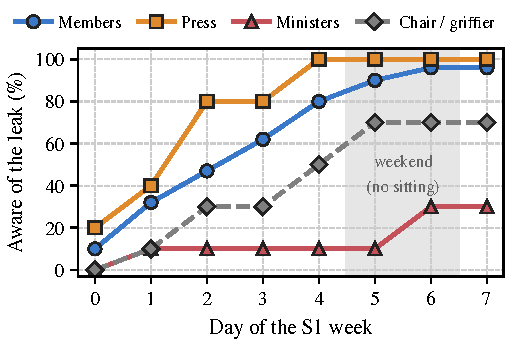
\includegraphics[width=\linewidth]{figure/fig_diffusion.pdf}
\caption{Leak diffusion (S1, $N{=}25$, 5-seed mean)}
\label{fig:diffusion}
\end{subfigure}\hfill
\begin{subfigure}[t]{0.485\textwidth}
\centering
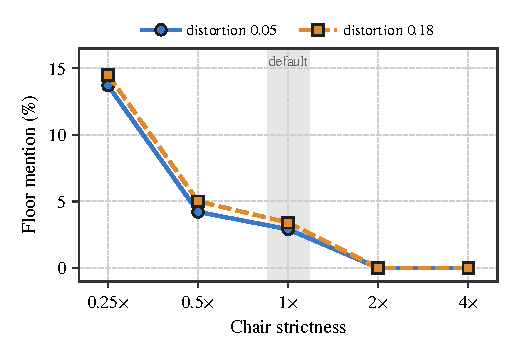
\includegraphics[width=\linewidth]{figure/fig_strictness.pdf}
\caption{Chair-strictness intervention (S3, 3-seed mean)}
\label{fig:cf}
\end{subfigure}
\caption{Corridor rumour and official record. (a)~A resignation rumour is
seeded with one member in the wandelgang. Members reach $32\%$ awareness
on day~1 and $96\%$ by day~7; the press is faster ($40\%$, then
$100\%$), and ministers lag ($10\%$, then $30\%$), as the transmission
probabilities in \S\ref{sec:communication} imply. Only $2\%$ of Handelingen lines
mention the leak. (b)~Floor mention of the leak against Chair strictness,
which lowers the heuristic allusion rate and, from $4\times$, drives
floor mention to zero.}
\Description{Two line charts side by side. Left: share of members, press,
ministers, and Chair or griffier aware of the leak over the S1 week, with
the weekend shaded. Right: share of floor lines mentioning the leak against
Chair strictness from 0.25 to 4 times the default, for two distortion
levels.}
\label{fig:s1s3}
\end{figure*}

\paragraph{Leak diffusion.} A single seeded leak reached $32\%$ of members
and $40\%$ of the press within one day and $96\%$ of members and all of
the press by day~7, whereas ministers reached $30\%$
(Figure~\ref{fig:diffusion}). This ordering follows from
the transmission rules in \S\ref{sec:communication}: in the wandelgang the
journalist hears a rumour with probability at least $0.55$ per encounter
and a minister with about $0.10$, and ministers spend their evenings in the
ministry rather than the wandelgang. The same leak appeared in only $2\%$ of simulated
Handelingen lines (Table~\ref{tab:interview}): an aware member alludes to
it on roughly one sitting day in twelve at the default Chair strictness,
and journalists cannot speak on the floor. Rumour hops embellished a
detail $16\%$ of the time, close to the distortion probability of $0.18$.

\paragraph{Mechanisms.} The affordance layer is what makes the
Handelingen selective (Table~\ref{tab:interview}). With it, the record
holds about one recognised speech per ten-minute step of the sitting week,
$205$ lines in all. Without it, as under GA, every member, minister, and the
journalist speaks at every step and is recorded: the record grows to
$4{,}876$ lines, and the journalist, one of 23 speakers, produces $4.3\%$
of it. No role transition is triggered in S1 (\S\ref{sec:gating}), so
--automaton is identical to the full model. Removing the rumour network
stops diffusion entirely, because rumours travel only on that channel;
floor speech does not pass them on.

\paragraph{Backbone.} Replacing the heuristic backend with
\texttt{gpt-4o-mini} leaves the selection diagnostics unchanged
(Table~\ref{tab:backbone}), as expected, since the model writes only what
agents say, not who speaks or where. In Smallville, by contrast, the
language model's disposition shaped behaviour and made agents overly
cooperative~\cite{park2023generative}. In \sys{}, the model's effect is
confined to content: floor mentions of the leak rise from $2\%$ to $10\%$,
because the model alludes to the rumour more readily than the heuristic
rule. The higher
embellishment rate ($20\%$ vs.\ $16\%$) and member awareness ($1.00$
vs.\ $0.96$) are not model effects, since rumour transmission and
distortion do not involve the language model; they reflect the different
seeds.

\begin{table}[t]
\caption{Selection-aware fidelity on held-out Tweede Kamer speeches
(1890--1899). Role JSD: lower is better. Journalist \% should be $0$.}
\label{tab:main}
\centering\small
\setlength{\tabcolsep}{4pt}
\begin{tabular}{lccc}
\toprule
Method & Role JSD $\downarrow$ & Journ.\ \% $\downarrow$ & Notes \\
\midrule
Archive (holdout) & --- & 0.0 & 20{,}166 speeches \\
Rule-ABM (1860--89 mix) & 0.001 & 0.0 & replay, no agents \\
GA~\cite{park2023generative} & 0.138 & 4.3 & ungated floor \\
\sys{} (naive calib.) & 0.131 & 1.8 & corridor counted \\
\sys{} (full) & 0.117 & \textbf{0.0} & 205 lines / week \\
\bottomrule
\end{tabular}
\end{table}

\paragraph{Macro fidelity.} The role mix is almost stationary between the
calibration and holdout decades (Rule-ABM JSD $0.001$), so simply
replaying the preceding thirty years matches \emph{who speaks}
(Table~\ref{tab:main}). The informative test is \emph{who must not
appear}. The archive never records a journalist; \sys{} reproduces that
zero, whereas GA and the affordance ablation do not. Naive calibration
(\S\ref{sec:calibration}) dilutes the official mix by treating wandelgang
talk as Handelingen and produces a $1.8\%$ press share that the archive
cannot contain. \sys{}'s role JSD ($0.117$) is higher than that of replay
because its record contains no Chair lines (\S\ref{sec:calibration}) and only
two ministers among 22 speakers: about $90\%$ of its lines are by members
and $10\%$ by ministers, against $64\%$, $18\%$, and $18\%$ for members,
government, and the Chair in the holdout. Among the agent-based
conditions, \sys{} has the lowest role JSD (GA $0.138$, naive calibration
$0.131$).



\paragraph{Interventions.} Floor mention falls from $8\%$ at
$0.25\times$ Chair strictness to $2\%$ at the default, $1\%$ at
$2\times$, and $0$ at $4\times$ (Figure~\ref{fig:cf}). This follows from how
strictness is encoded (\S\ref{sec:experiments}): it lowers the rate at
which aware members allude to the rumour and, from $2\times$, halves or
quarters the number of recognised speeches. Corridor distortion, which
changes only the content of rumours, leaves the rate unchanged.

\paragraph{Presentism audit.} A nine-term English check finds no modern
term in the S1 records, which consist mostly of attested excerpts. In the
presentism audit every record line is model text
(Table~\ref{tab:presentism}). Under GA, $10.5\%$ of record lines contain
a modern term, $1.4\%$ an adversarial marker, and $49.9\%$ a consensus
cue (archive: $0.0\%$, $28.9\%$, $0.6\%$). The period prompt halves
modern vocabulary and cuts modern spelling from $93\%$ to $27\%$. The
\sys{} world lowers modern vocabulary to $3.6\%$, within the prompt-only
interval, raises adversarial markers to $10.6\%$, and lowers consensus
cues to $26.2\%$. Retrieval removes modern forms of address ($37\%$ to
$0\%$) without verbatim copying, and the filter brings modern vocabulary
to $0.3\%$; on the lexicon half the filter never sees, the rate stays at
$0.3\%$, so the filter removes the terms it targets rather than modern
language in general. No condition reaches the archive's register. In
interviews, $13$--$18\%$ of answers contain a modern term in every
condition until the filter ($2.7\%$), and self-description errors are
$4\%$ in all four conditions.

\begin{table}[t]
\caption{Presentism audit on simulated Handelingen lines
(\texttt{gpt-4o-mini}, 3 seeds; every line is model text). Shares of
distinct completions with a modern term, an adversarial marker, or a
consensus cue; brackets give 95\% cluster-bootstrap intervals.}
\label{tab:presentism}
\centering\small
\setlength{\tabcolsep}{2.5pt}
\begin{tabular}{lccc}
\toprule
Condition & Modern \% & Adversarial \% & Consensus \% \\
\midrule
Handelingen 1890--1899 & 0.0 & 28.9 & 0.6 \\
GA~\cite{park2023generative} & 10.5 [8--14] & 1.4 [1--2] & 49.9 [48--51] \\
GA + period prompt & 5.0 [2--9] & 7.2 [6--8] & 34.2 [30--39] \\
\sys{} world & 3.6 [2--6] & 10.6 [7--14] & 26.2 [21--31] \\
\sys{} + guards & \textbf{0.3} [0--1] & 8.8 [7--11] & 22.9 [17--29] \\
\quad before filter & 2.3 [0--5] & 8.9 [7--11] & 23.7 [17--30] \\
\bottomrule
\end{tabular}
\end{table}

\paragraph{Historian review.} The rater passed both attention checks,
which planted obvious anachronisms (a Twitter livestream; ``I am a large
language model''). On the remaining pairs, \sys{} outranked the
Smallville-style ablation on both criteria (17--8--11 for believability,
12--5--19 for procedure; Table~\ref{tab:historian},
Appendix~\ref{app:historian}).
Ties were more frequent for procedure than for believability, consistent
with both systems being prompted about recognition. The standing-order
vignettes matched the intended $\pi$: a journalist on the floor is out of
order and off the record, as is an unrecognised interruption, whereas
wandelgang talk is in order but not part of the Handelingen.
Appendix~\ref{app:historian} lists the changes the rater requested, the
OCR-card results, and the resulting roster correction.



%% =====================================================================
\section{Discussion}
\label{sec:discussion}

\paragraph{What a sandbox can claim.} \sys{} produces \emph{sufficiency}
evidence: mechanisms that, under explicit assumptions, generate patterns
consistent with the Handelingen. Several patterns reported here, including
the order in which roles learn of the leak and the effect of Chair
strictness, follow directly from transmission and allusion rules that we
set by hand. Their value lies in making these assumptions explicit and
showing how they combine over a week of sittings, not in emerging
unprompted. No run can establish what a historical member thought:
agents' utterances are model artefacts, not recovered voices. The sandbox instead makes
historians' assumptions about procedure and selection explicit and
manipulable, and it generates hypotheses for further archival work in
committee minutes, private correspondence, and the press.

\paragraph{Limitations.} The 1814--1899 slice is OCR-noisy, speaker
strings do not identify unique persons, and 1890s party labels denote
kamerclubs rather than mass parties. The Binnenhof is a composite, and the
journalist is a synthetic observer. S1 is a 25-agent Tweede Kamer week, so
it cannot match the role mix of a full chamber, and it runs no Eerste Kamer
sitting even though senate tiles and affordances exist in the world. A
single historian ranked interviews generated at the end of each run rather
than in live sessions, and logged interventions other than opening a
sitting do not yet change what agents do. The implementation is also simpler
than the Generative Agents architecture: it has no memory ranking,
reflection, or model-driven planning; conversations are single remarks;
agents hear the content of floor speeches only in the presentism audit;
and archival retrieval and the anachronism filter are active only there,
so the S1--S3 records consist mostly of attested excerpts
(\S\ref{sec:experiments}). We release seeds, configurations, and the
DutchParl parser.

%% =====================================================================
\section{Ethical Considerations}
\label{sec:ethics}

\paragraph{Commitments for a parliamentary sandbox.}
(1)~\emph{Public persons in public roles.} Agents are seeded from
attested speakers in CC0 proceedings; we do not invent private lives,
families, or unrecorded interiors.
(2)~\emph{No gamification.} There is no playable persona, no score, and
no first-person control of the Chair or of ministers.
(3)~\emph{Provenance.} All simulated text, including the simulated
Handelingen, is labelled and kept separate from the archival XML.
(4)~\emph{Procedure over psychology.} Claims concern standing orders,
selection, and diffusion, not what a named member ``really thought''.
(5)~\emph{Consultation.} The project is designed with historians of
Dutch politics. The labelling reported here was carried out with informed,
task-specific consent, and the rater could skip any item.
(6)~\emph{Copyright.} The corpus is released under
CC0~\cite{marx2012dutchparl}, and Auteurswet art.~11 places official
proceedings outside copyright.

%% =====================================================================
\section{Conclusion}
\label{sec:conclusion}

LLM agents carry present-day bias, and simulating the past makes it
visible. \sys{} counters this bias outside the language model: attested
speakers and their speech supply the agents, and standing orders encoded
in the world decide who may act and what is recorded. This procedure held
regardless of the backbone: journalists never entered the simulated
Handelingen, whereas without the floor rules they produced $4.3\%$ of it
under both the heuristic backend and \texttt{gpt-4o-mini}. The record also
diverged from what parliament knew: a rumour known to almost all members
appeared in only $2\%$ of official lines, so silence in the record does
not imply ignorance. Present-day bias in LLM agents thus lies in the worlds they
are placed in as well as in what they say. Encoding the period's
institutions removes the former. For the latter, a period prompt, the
world, and archival retrieval with filtering lower modern vocabulary in
model-written records from $10.5\%$ to $0.3\%$, but the register stays far
more consensual than in the 1890s Handelingen.

%% =====================================================================
\begin{acks}
Anonymised for review.
\end{acks}

\bibliographystyle{ACM-Reference-Format}
\bibliography{references}

\appendix

\section{Sandbox step}
\label{app:alg}
Algorithm~\ref{alg:step} summarises one ten-minute step of \sys{} as
implemented in the runs reported here.

\begin{algorithm}[t]
\caption{One sandbox step of \sys{}}
\label{alg:step}
\small
\begin{algorithmic}[1]
\For{each agent $i$, in roster order}
  \State $o_i \gets$ \Call{Perceive}{$\ell_i^t$} $\cup$ \Call{Inbox}{$i$} \Comment{place, sitting, floor, rumours}
  \State $M_i \gets M_i \cup o_i$; add places named in rumours to $\mathcal{T}_i$
  \State move to \Call{Schedule}{$\rho_i^t$, clock, sitting} if permitted
  \State $a_i \gets$ \Call{RuleAction}{$\rho_i^t,\ell_i^t$, sitting, floor holder}
  \If{$a_i\notin\mathcal{C}(\rho_i^t,\ell_i^t,t)$}
     \State $M_i \gets M_i\cup\{\textsc{Refusal}(a_i)\}$;\; $a_i\gets\textsc{wait}$
  \EndIf
  \State \textbf{if} $a_i=\textsc{speak}$ \textbf{then} $u_i \gets$ \Call{Utter}{persona, recent $M_i$}
  \State execute $a_i$ \Comment{e.g.\ open, adjourn, recognise}
\EndFor
\State \Call{Encounters}{}: remarks and rumour hops at fixed hours
\State $Y^{t}\gets Y^{t-1}\cup\{u_i : a_i=\textsc{speak}$, $i$ recognised on the floor$\}$
\State apply scheduled sitting events; advance the clock by ten minutes
\end{algorithmic}
\end{algorithm}

\section{Seed and utterance examples}
\label{app:examples}
Each agent is seeded with a short persona and up to three excerpts of the person's actual public speech (\S\ref{sec:personas}). The agent for Abraham Kuyper, leader of the Anti-Revolutionary Party, receives the persona below
and, among its excerpts, the passage that follows it, taken from the
sitting of 20 November 1896 with OCR errors preserved:
\begin{quote}\small\ttfamily\raggedright
De heer Kuyper is Kamerlid der Tweede Kamer (1899-1900). Partij: nl.p.arp.
Het publieke woord, zoo het op de vloer klinkt, is tot den Voorzitter
gericht.\par\smallskip
Mynhee r de Voorzitter! Aa n de koffie en het djatihout besteedde de Kamer
een niet onbelangrijk deel van den beschikbaren parlementairen tijd. E n
ongetwijfeld zyn ook die materieele belangen van gewicht [\ldots]
\end{quote}
(``Mr Kuyper is a member of the Tweede Kamer (1899--1900). Party:
Anti-Revolutionary. Public speech, as it sounds on the floor, is addressed
to the Chair.'' ``Mr Chairman! The Chamber spent no small part of the
available parliamentary time on coffee and teak. And these material
interests are no doubt also of weight [\ldots]'')

On the fifth day of one
\texttt{gpt-4o-mini} run (seed~19), de Beaufort said to the journalist in
the wandelgang:
\begin{quote}\small
Waarde Verslaggever, ik kan u niet ontkennen dat de geruchten omtrent het
ministerie der Koloniën ons allen bezighouden. Het is eene tijd van
spanning, en ik vrees dat de Minister van Koloniën, de heer Goeman
Borgesius, over de begroting der Indische afdeeling wel eens in een
moeilijke positie mag verkeren. Laat ons hopen dat de wijsheid zal
zegevieren in deze aangelegenheid.
\end{quote}
(``Dear Reporter, I cannot deny that the rumours about the Ministry of
Colonies occupy us all. It is a time of tension, and I fear that the
Minister of Colonies, Mr Goeman Borgesius, may well find himself in a
difficult position over the budget of the Indies department. Let us hope
that wisdom prevails in this matter.'') The remark passes on the rumour in
period-flavoured Dutch but names Goeman Borgesius, the Minister of the
Interior, as Minister of Colonies. Such factual slips remain in the
language model's text, whereas who may speak where, and what is recorded,
is fixed by the world.



\section{Calibration objective}
\label{app:calib}
Calibration fits $\theta$ on the simulated Handelingen $Y$:
\begin{equation}
\theta^\star=\arg\min_{\theta}\;\sum_{f\in F} w_f\,
D\!\left(\tilde P^{\theta}_{\text{sim},f},\,P_{\text{arch},f}\right),
\label{eq:calib}
\end{equation}
over marginals $F$ (house, role, party, topic, speech length, month),
using Jensen--Shannon divergence for categorical features and $W_1$ for
ordinal ones, with 1860--1889 reserved for calibration and 1890--1899
held out. The runs reported in \S\ref{sec:results} use the default
parameters and do not solve Eq.~\eqref{eq:calib}.

\section{Simulated and real silence}
\label{app:silence}
In Figure~\ref{fig:teaser}, the
Handelingen page records a recognised speech on the East Indies budget,
while the resignation leak, the journalist's notes, and the minister who
has not yet heard of it remain invisible to the stenographer. The
simulated Handelingen thus reproduces the structural silences of the real
one~\cite{trouillot1995silencing}, and the sandbox makes the gap between
them inspectable.

\section{Interface and researcher controls}
\label{app:interface}
\paragraph{Actions and their display.} At each step, every agent takes one
action from a fixed repertoire: move, speak, request the floor, talk, take
notes, recognise a speaker, open or adjourn the sitting, record, or wait.
The action follows from the agent's role, its location, and the sitting
schedule, and is then checked against the affordance layer. The interface
shows each action as an emoji above the agent's token, such as a
microphone for floor speech, a raised hand for a request for the floor,
and a speech balloon for conversation, together with the agent's current
utterance in a bubble; clicking the agent opens the inspector
(Figure~\ref{fig:teaser}, right). Smallville uses a language model to
turn each action into emojis; in \sys{} the mapping from action to emoji
is fixed.



\paragraph{Partial spatial knowledge.} Each agent holds its own subtree
$\mathcal{T}_i\subseteq\mathcal{T}$. Smallville agents extend their subtree
only by visiting places; in \sys{}, agents can also learn nodes from
\emph{dialogue}, so a newly elected member may know that Afdeeling~A is
meeting without having been there. The subtree records which places an
agent knows and how it learned them (initial knowledge, a visit, or
dialogue). Object states that the agent perceives on site enter its memory
stream as observations rather than being stored in the tree. In the
reported runs the subtree is shown in the inspector but does not restrict
movement, which follows the schedule above.

\paragraph{Researcher controls.} The sandbox supports five forms of
interaction, all of which are logged. \emph{Inspect} shows an agent's
role, function, party, location path, current action and utterance, last
refusal, and eight most recent memories (Figure~\ref{fig:teaser}, right).
\emph{Interview} pauses the world and poses a question, which the agent
answers from its recent memories without writing the exchange back
(\S\ref{sec:eval-interview}). \emph{Inner voice} adds a memory, such as
``You heard in the wandelgang that the minister will resign''; it can
reach the language model's prompt but not the rumour channel.
\emph{Edit object} changes an object state, for example closing the
speaker list; agents perceive the new state, but no rule reads it.
\emph{Inject event} records a named event such as a cabinet crisis; in
the current version only opening a sitting changes the world. No agent can be controlled in
the first person.

\section{Historian review details}
\label{app:historian}
\begin{table}[t]
\caption{TrueSkill ranking of pause-and-interview answers by one historian
(\sys{} with LLM vs.\ Smallville-style GA). Attention checks passed: $2/2$.
Higher $\mu$ is better; $\sigma$ is the posterior uncertainty. Pairwise
(win--loss--tie): believability 17--8--11, procedure 12--5--19. One further
pair, from an earlier version of the task, was left unranked with a
written comment (``Kamerlid der Tweede/Eerste Kamer'', not ``MP'').}
\label{tab:historian}
\centering\small
\setlength{\tabcolsep}{3.5pt}
\begin{tabular}{lcccc}
\toprule
Condition & $\mu_{\text{bel}}$ & $\sigma$ & $\mu_{\text{proc}}$ & $\sigma$ \\
\midrule
\sys{} (full, LLM) & \textbf{28.3} & 1.8 & \textbf{27.8} & 2.2 \\
GA~\cite{park2023generative} & 21.7 & 1.8 & 22.2 & 2.2 \\
\bottomrule
\end{tabular}
\end{table}
The rater
asked us to separate the griffier from the stenographer, to let Kamerleden
speak in afdeelingen without plenary recognition, to let ministers talk in
the wandelgang, and, in the comment that most changed the world, to stop
treating the Tweede and Eerste Kamer as one chamber. On the OCR speaker
cards, $27/40$ names were accepted, with a mean OCR quality of $3.8/5$.
Party was the weakest field ($18$ yes / $13$ no / $7$ uncertain) because
1890s ``parties'' were kamerclubs (parliamentary factions) that could
merge, as the Bahlmannianen and Schaepmannianen did into a Roman Catholic
bloc in 1896. Following this review, S1 seeds the Pierson cabinet in office
at $t_0$ (Cremer at Colonies, Goeman Borgesius at Interior, Gleichman in
the chair, Arntzenius as griffier) and drops van Houten, Sprenger van Eyk,
and Gerritsen, who did not hold those posts in December 1899. The heuristic
runs behind Tables~\ref{tab:interview} and~\ref{tab:main}, the heuristic
rows of Table~\ref{tab:backbone}, and Figure~\ref{fig:s1s3} use the
corrected cabinet. The \texttt{gpt-4o-mini} runs, including the interviews
ranked in Table~\ref{tab:historian} and the remark in
Appendix~\ref{app:examples}, predate the correction; minister identity does
not change who may speak. Appendix~\ref{app:day} traces a day of an earlier
heuristic run with the corrected cabinet. The presentism audit
(Table~\ref{tab:presentism}) uses the current code, in which synthetic
cards are excluded from the roster and the corridor object is a kamerclub
circular.

\section{Sandbox objects and corpus slice}
\label{app:tables}
Table~\ref{tab:objects} lists the stateful objects of the Binnenhof, and
Table~\ref{tab:corpus} summarises the slice of the proceedings used to
seed \sys{} (\S\ref{sec:pipeline}).

\begin{table}[H]
\caption{Representative sandbox objects and their states.}
\label{tab:objects}
\centering\footnotesize
\setlength{\tabcolsep}{3pt}
\begin{tabular}{lll}
\toprule
Object & States & Changed by \\
\midrule
Gavel & resting, opening, adjourned & chair \\
Speaker list & empty, open, closed & chair, griffier \\
Kamerstuk & tabled, in debate, voted, withdrawn & government, chair \\
Stenograph & idle, recording, paused & stenographer \\
Voting box & closed, open, counted & chair, griffier \\
Press-gallery desk & empty, occupied & journalist \\
Kamerclub circular & none, circulating, spent & members \\
\bottomrule
\end{tabular}
\end{table}

\begin{table}[H]
\caption{Working slice of DutchParl (1814--1899) used to seed \sys{}. The
S1 speaker pool is the first 80 Tweede Kamer sittings of 1896--1899 and
holds 205 distinct speaker strings.}
\label{tab:corpus}
\centering\small
\begin{tabular}{lrrr}
\toprule
 & Sittings & Speeches & Years \\
\midrule
Tweede Kamer (commons) & 6{,}340 & --- & 1814--1899 \\
Eerste Kamer (senate) & 2{,}036 & --- & --- \\
Other / early Staten-Generaal & 369 & --- & --- \\
\midrule
All sittings in slice & 8{,}745 & 138{,}214 & 86 years \\
\quad with $\geq$1 \texttt{speech} & 7{,}348 & 138{,}214 & --- \\
Member identifiers & 852 & --- & --- \\
S1 speaker pool (TK) & 80 & --- & 1896--1899 \\
Holdout TK 1890--1899 (S2) & 731 & 20{,}166 & --- \\
Calibration TK 1860--1889 (S2) & 2{,}821 & 72{,}112 & --- \\
\bottomrule
\end{tabular}
\end{table}

\section{A day in the sandbox}
\label{app:day}
\begin{figure*}[t]
\centering
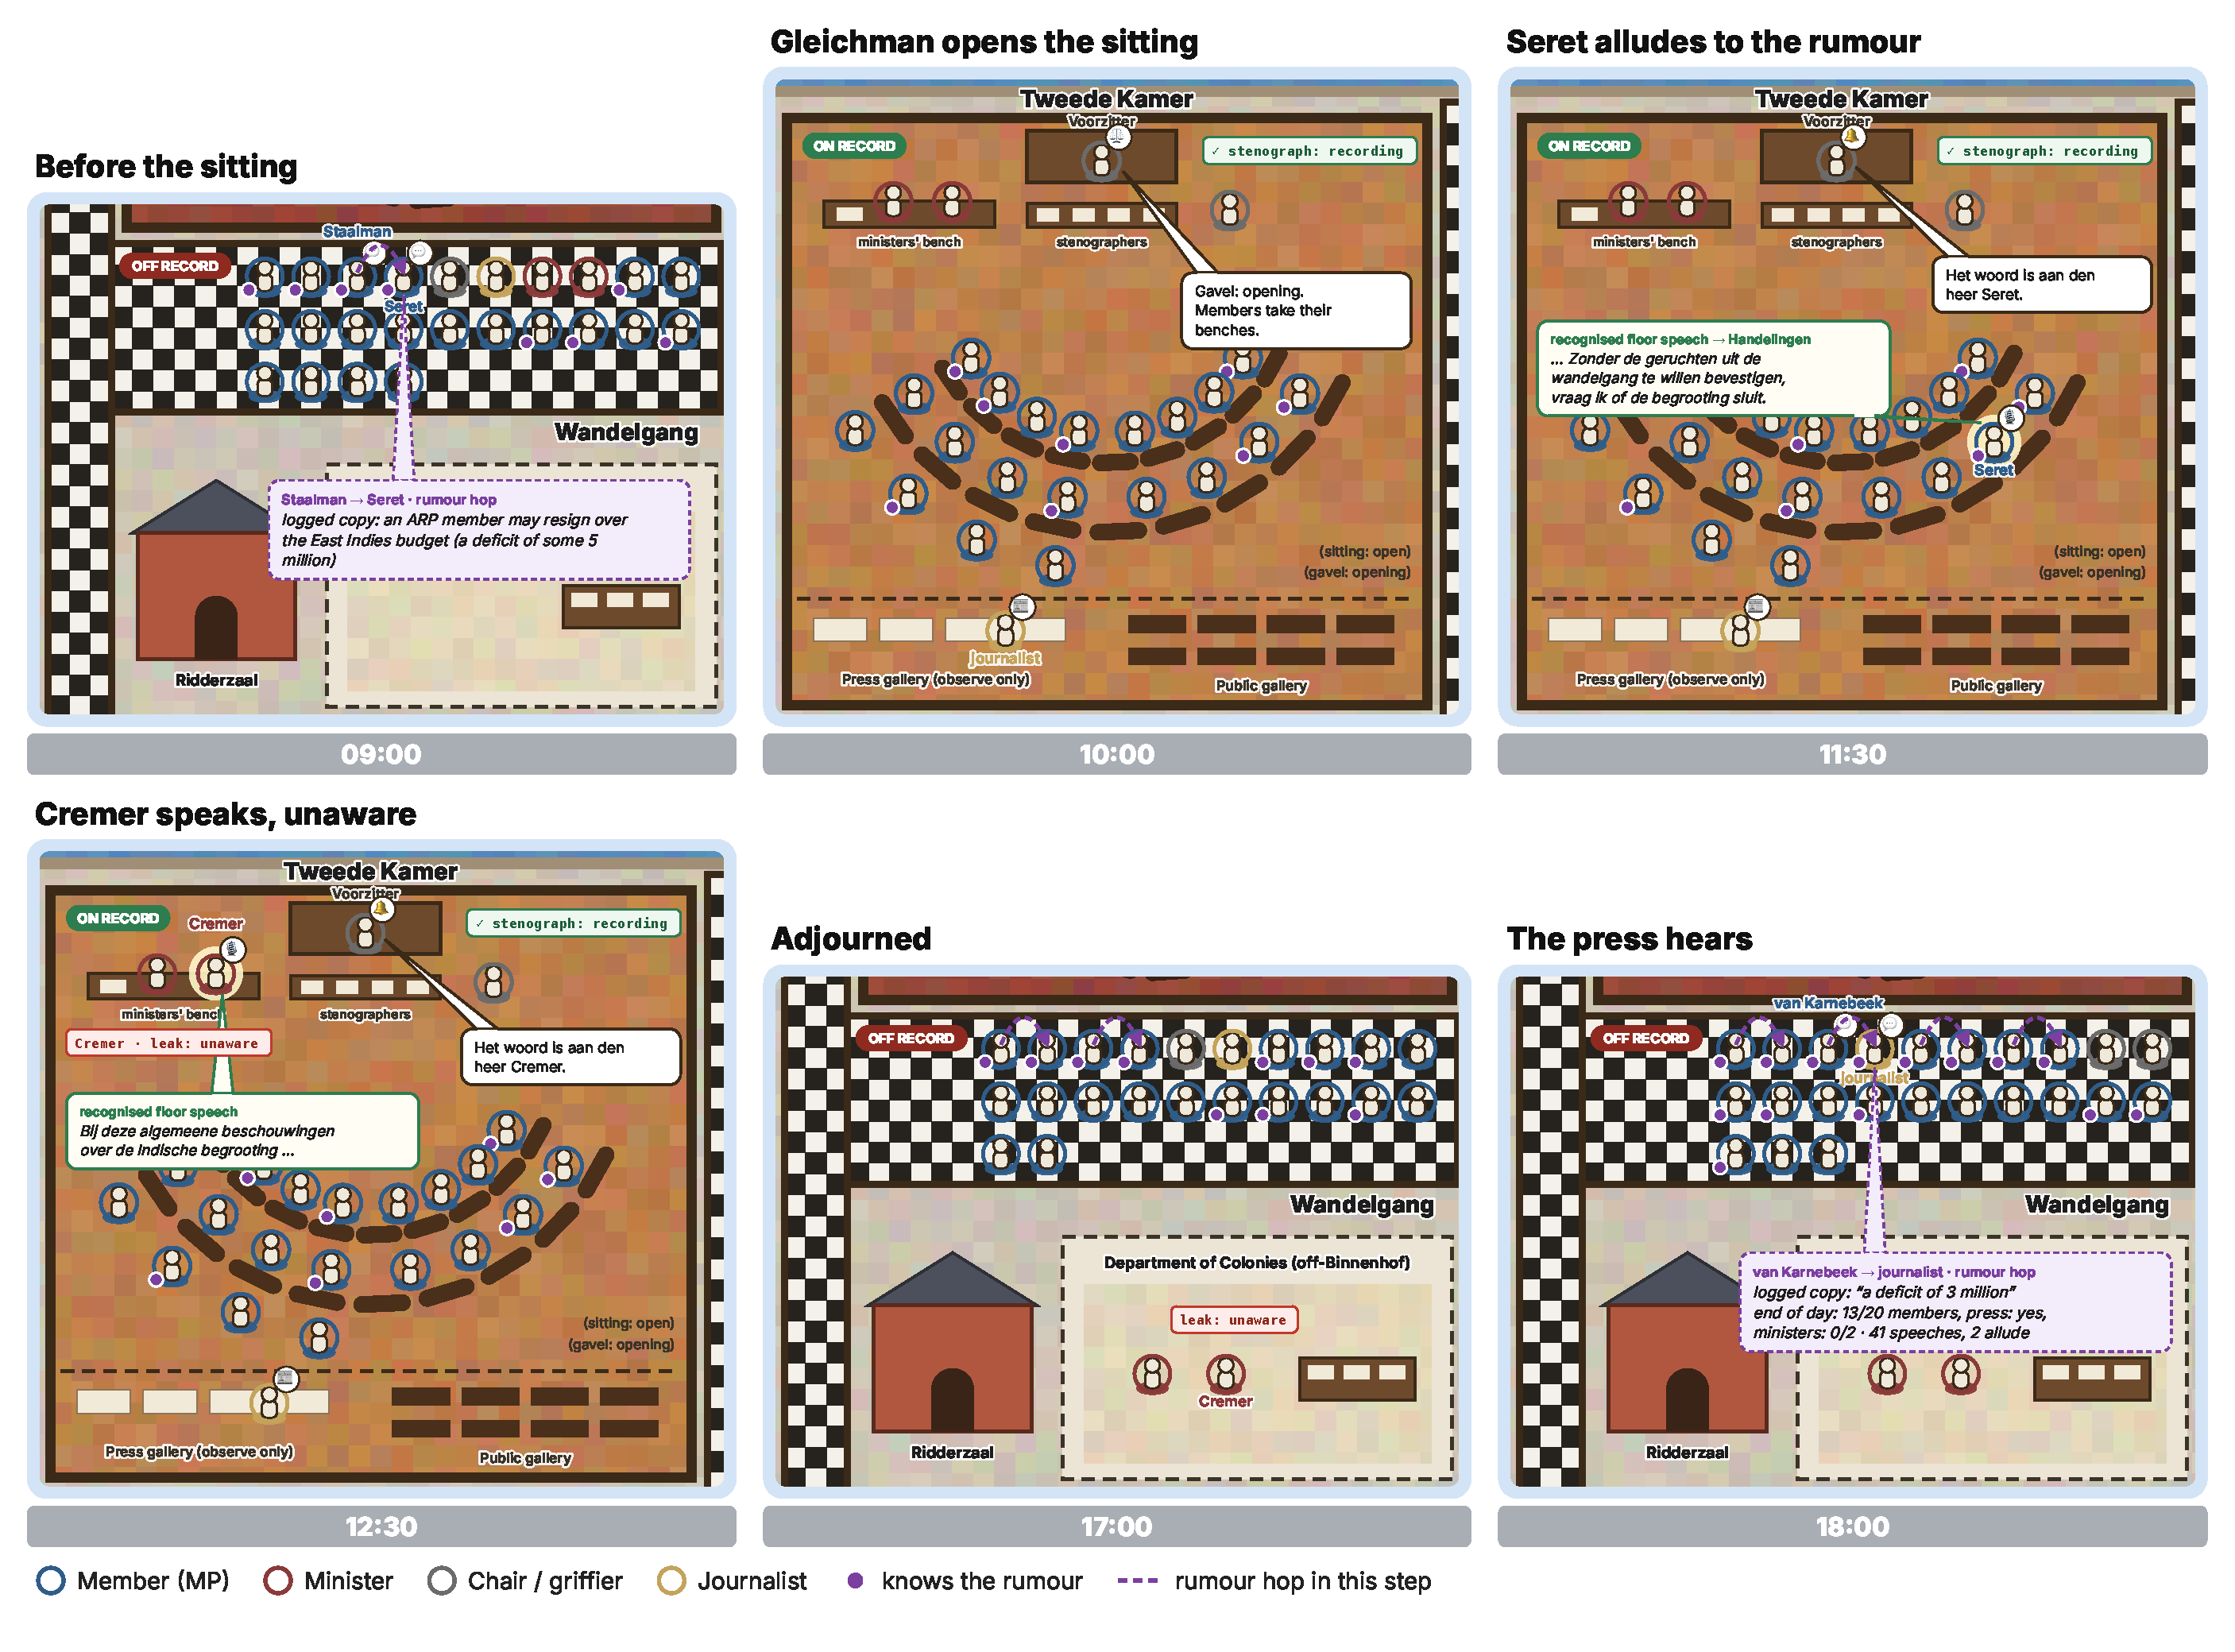
\includegraphics[width=\textwidth]{figure/day_timeline.pdf}
\caption{A day in \sys{}: Wednesday 20 December 1899 in an earlier
heuristic S1 run with the corrected cabinet (seed~19;
Appendix~\ref{app:historian}), drawn in the style of Figure~\ref{fig:teaser} from the
logged state at six moments. Rooms, roles, actions, awareness (purple
dot), rumour hops, object states, and utterances come from the run;
positions within a room are a layout choice, since the simulation records
only the room. Staalman passes the rumour to Seret before the sitting; Seret
alludes to it on the floor and the stenographer records the speech;
Cremer, the Minister of Colonies, speaks without having heard it and
withdraws to his department after the adjournment; the journalist hears
the rumour in the wandelgang at 18:00.}
\Description{Six crops of the Binnenhof sandbox map at 09:00, 10:00,
11:30, 12:30, 17:00, and 18:00. Agent tokens carry role-coloured rings and
a purple dot when they know the rumour; dashed purple arcs mark rumour
hops, and speech bubbles quote utterances from the run.}
\label{fig:day}
\end{figure*}

To show how the rules of \S\ref{sec:agents} play out, we trace Wednesday 20 December 1899, the third day of an earlier heuristic S1
run with the corrected cabinet (seed~19; Figure~\ref{fig:day}). At 09:00, before the sitting, members gather in the
wandelgang, and Staalman passes the resignation rumour to Seret. The
provenance log records Seret's copy with one fact changed: ``an ARP
member may resign''. At 10:00 Gleichman opens the sitting. Members take
their benches and ask for the floor, the journalist moves to the
press-gallery desk and takes notes, and the Chair gives the floor in
rotation. When Seret is recognised at 11:30, his speech consists of the
opening of an attested excerpt, cut at 220 characters, followed by the
fixed allusion, and the stenographer records it:
\begin{quote}\small
Mijnheer de Voorzitter! Ik kan mij geheel aansluiten bij hetgeen in de
laatste plaats door den Minister is gezegd ten aanzien vau het amendement
van den heer Mackay. [\ldots] Zonder de geruchten uit de wandelgang te
willen bevestigen, vraag ik of de begrooting sluit.
\end{quote}
(``Mr Chairman! I fully concur with what the Minister last said about
Mr Mackay's amendment. [\ldots] Without wishing to confirm the rumours
from the wandelgang, I ask whether the budget balances.'') At 12:30
Cremer, the Minister of Colonies, speaks on the Indies budget from the
ministers' bench without having heard the rumour about himself. Seret
speaks again at 15:10 with the same allusion. Gleichman adjourns at
17:00; the members return to the wandelgang, and Cremer withdraws to the
Department of Colonies. In the encounters at 17:00 and 18:00, five more
members hear the rumour, and van Karnebeek passes it to the journalist,
whose logged copy now names a deficit of 3 million. By the end of the day,
13 of the 20 members and the journalist know the rumour, neither minister
does, and the day's Handelingen hold 41 speeches, two of them with the
veiled allusion.

\end{document}
